\chapter{Introdução}\label{CAP:introducao}

Este documento descreve o desenvolvimento de um sistema para captação e análise de dados referentes à direção de um motorista.

A ideia básica é coletar dados de sensores já presentes em carros modernos através da porta OBD-II, que utiliza um padrão internacional de disponibilização de informações referentes a um carro\textsuperscript{[2]}, assim como informações disponibilizadas por um celular (geolocalização) e armazená-los em uma plataforma de dados, onde poderão ser posteriormente analisados.

\section{Motivação}

Qual o perfil de direção de um motorista? Como categorizar os condutores segundo um critério claro?

Buscando responder essas perguntas e, consequentemente, entender as características de pessoas ao volante, este trabalho propõe-se a criar uma infraestrutura de captura e análise de dados em automóveis de uso pessoal.

Com base nos dados de aceleração, é possível classificar o estilo de direção, identificar comportamentos perigosos, e até mesmo antecipar a necessidade de manutenção do veículo. A integração da análise da aceleração em sistemas de perfil de direção não apenas contribui para a segurança do veículo, mas também possibilita a personalização de feedbacks e sugestões ao motorista, promovendo uma condução mais eficiente e segura.

As informações recolhidas foram armazenadas em uma plataforma de nuvem, protegidas por algum nível de segurança, implementado neste mesmo projeto e, por fim, foram analisadas para gerar conclusões interessantes sobre o modo de dirigir de cada participante do estudo.
	
Uma pesquisa preliminar sobre o assunto revelou que já existe uma patente para um produto parecido; ela foi registrada em 2013 e avalia o desempenho de um motorista a partir de dados pré-coletados de parâmetros relevantes à condução do carro \textsuperscript{[1]}.

\section{Objetivo}

Este trabalho procura criar uma plataforma de disponibilização e captura de dados em um carro, coletando as informações \textit{in loco} e apresentando estatísticas relevantes derivadas do que foi coletado.

Para isso, fez uso da infraestrutura já presente em carros atuais. Conforme pode ser visto na imagem \ref{fig:sensors_car}, alguns carros podem ter dezenas de sensores embarcados dentro de si.


\begin{figure}[hp]
    \centering
    
    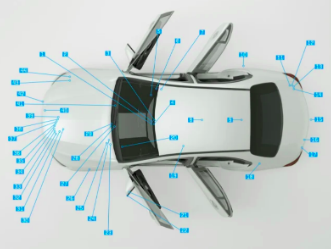
\includegraphics[]{figures/sensores_carro.png}
    
    \caption{Sensores estão presentes em um carro atual na ordem de dezenas\textsuperscript{[2]}.}
    
    \label{fig:sensors_car}
\end{figure}

Essas informações foram complementadas com o uso de um \textit{smartphone}. Já que no smartphone foi possivel capturados os dados referentes a aceleração.

A análise da aceleração desempenha um papel crucial na avaliação do comportamento do motorista em sistemas de rastreamento de veículos. Ao monitorar padrões de aceleração, é possível extrair informações valiosas sobre a condução, como a suavidade nas transições de velocidade, a resposta a mudanças nas condições de tráfego e o grau de agressividade na condução. A aceleração fornece insights sobre a habilidade do motorista em manter uma condução estável e prever suas ações em situações específicas. 

A coleta de dados foi feita, a princípio, a partir de ensaios em carros reais feitos por uma quantidade seleta de pessoas, que pode ser expandida para resultados mais precisos na análise posterior.

Os dados coletados foram passados para o serviço de nuvem da AWS, usando conexão à \textit{internet}, caracterizando uma aplicação IoT.
	
Do lado da nuvem, foi possível utilizar os dados de cada usuário de forma anônima, para diagnosticar condutor e possivelmente gerar \textit{insights} sobre como a pessoa poderia melhorar.

 
\section{Justificativa}
% ROMEO e PIRES [GIT]
% Pq o trabalho é importante?
No ano de 2021, 11647 pessoas morreram em acidentes de trânsito no Brasil\textsuperscript{[6]}, além disso, no mundo inteiro morrem 1,35 milhão de pessoas em média, todos os anos\textsuperscript{[7]}, número comparável às mortes por Covid 19 até abril de 2022\textsuperscript{[8]}.

Levando-se em conta esses fatos, é simples entender a relevância deste projeto, pois ele define métricas importantes para classificação da conduta de motoristas, as quais podem ser usadas justamente para evitar acidentes e, portanto, preservar a vida humana.

É possível que no futuro os carros não sejam mais dirigidos por humanos ou que atuem por conta própria na maior parte das situações. Prevê-se, inclusive, que carros com pelo menos nível 4 de automação comecem a se popularizar em 2025 \textsuperscript{[9]}.

Dessa forma, embora o fator humano venha a ser menos relevante para os acidentes do futuro, é preciso também haver métricas para classificar a condução dos veículos autônomos.

Este projeto tem, portanto, extrema relevância, pois é uma possível ferramenta para diminuir as mortes no trânsito, seja causada por pessoas ou por carros autônomos.

\section{Organização do trabalho}
Os próximos capítulos explicitarão como o trabalho foi planejado a partir de seus requisitos e das tecnologias envolvidas.

O projeto consistiu em integrar a porta OBD-II de qualquer carro com a plataforma de armazenamento de dados que foi criada.

Para isso, o Capítulo 2 faz uma breve apresentação dos conceitos usados neste projeto. O Capítulo 3, por sua vez, traz as etapas de desenvolvimento do trabalho e o Capítulo 4 mostra quais requisitos foram definidos para o sistema. Além disso, o desenvolvimento inicial do trabalho é descrito no Capítulo 5. Por último, o Capítulo 6 traz as considerações finais com uma breve discussão das conclusões do trabalho, assim como contribuições e sugestões para a continuidade dele.